\clearpage\chapter{Piecewise Functions}
Piecewise functions are a kind of break from the composite and inverse functions we've been working on up to this point. Piecewise functions are best used when the formula deciding the input changes after a certain $x$ value. Examples often used with piecewise functions include tax brackets, shipment/delivery price changes, discounts dependent on age, etc.

Before hopping into any examples, I think it's best to get acquainted with what a piecewise function looks like and how to graph it. Consider the below piecewise function:
\[
f(x) = 
\begin{cases}
    x & 0 \le x \le 4 \\
    -(x - 4) + 4 & 4 < x \le 8 \\
    \frac{x - 8}{2} & x > 8
\end{cases}
\]
What do you think this looks like? I've written the explanation of this on the next page, so take a moment to think about what happens before moving on.
\begin{itemize}
    \item Why are there compound inequalities next to equations?
    \item Why are some of the inequalities $<$ and others $\le$?
    \item What's up with that $x > 8$ in the bottom row? Why is it different?
    \item Could these compound inequalities by written in some other way?
\end{itemize}
\clearpage
\section{Describing Piecewise Functions}
Alright. Here it is.

The $f(x)$ is the name of the function, as is the case with any other function. It is set equal to a curly bracket containing cases.

Each row first identifies and equation and next by an interval that the equation applies within.

Using the above function as an example:
\[
x \qquad \qquad 0 \le x \le 4
\]
means to say that the equation $y = x$ applies for all $x$ values between $0$ and $4$.
\[
-(x - 4) + 4 \qquad \qquad 4 < x \le 8
\]
means to say that the equation $y = -(x - 4) + 4$ applies for all $x$ values between $4$ and $8$ excluding $4$. The value $x = 4$ is excluded because it's already accounted for in the previous domain.
\[
\frac{x - 8}{2} \qquad \qquad x > 8
\]
means to say that the equation $\frac{x - 8}{2}$ applies for all $x$ values that are greater than $8$. Again, the inequality is not $x \ge 8$ because the value $x = 8$ was accounted for in the previous domain.

The inequality $x > 8$ could be written as $8 < x < \infty$ so that it matches the other inequalities.

The piecewise function could also be rewritten using interval notation, like so:
\[
f(x) = 
\begin{cases}
    x & x \in [0, 4]\\
    -(x - 4) + 4 & x \in (4, 8] \\
    \frac{x - 8}{2} & x \in (8, \infty)
\end{cases}
\]
\clearpage
This piecewise function produces the graph below:
\begin{figure}[ht]
    \centering
    \caption{Graph Of Piecewise Function $f(x)$}
    \label{fig:Piecewise Example 1}
    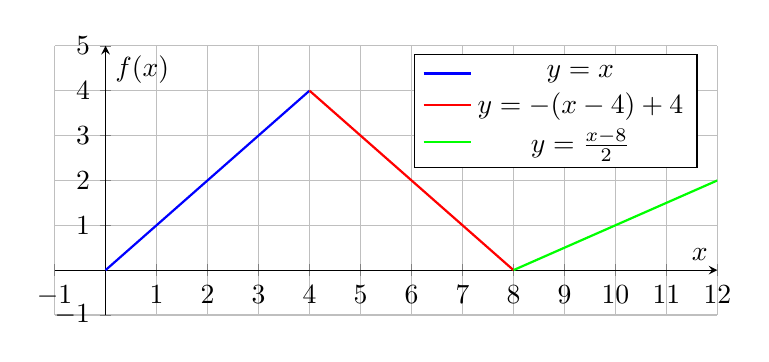
\begin{tikzpicture}
        \begin{axis}[
            axis lines = middle,
            xlabel = $x$, ylabel = {$f(x)$},
            xmin = -1, xmax = 12,
            ymin = -1, ymax = 5,
            xtick distance={1}, ytick distance={1},
            width = 10cm, height = 5cm,
            grid = both,
            legend pos = north east, % Positions the legend
        ]
            \addplot[blue, thick, domain=0:4, samples=100] {x};
            \addlegendentry{$y = x$}

            \addplot[red, thick, domain=4:8, samples=100] {-(x - 4) + 4};
            \addlegendentry{$y = -(x - 4) + 4$}

            \addplot[green, thick, domain=8:12, samples=100] {(x - 8) / 2};
            \addlegendentry{$y = \frac{x - 8}{2}$}
        \end{axis}
    \end{tikzpicture}
\end{figure}
\section{Example with Piecewise Functions}
Now that we know what a piecewise function \textit{is}, let's look at an example of where it may be used.

"Totally real bank name" gives money out for free. If we say that $x$ represents the number of hours that have passed, then:
\begin{itemize}
    \item The first $4$ hours, represented as $0 \le x \le 4$, \$$10$ are given out per hour.
    \item The following $9$ hours, represented as $4 < x \le 13$, \$$7$ are given per hour.
    \item Every hour after that, represented as $x > 13$ or $13 < x < \infty$, \$$5$ are given out per hour.
\end{itemize}
Instead of writing each and every case, we can use a piecewise function to set all three cases equal to a function $f$. This function will output the amount of money given out after $x$ hours.
\clearpage
\subsection{Potential Trap}
We should be careful when constructing such a function, however. We can't simply call the equatoins $10x$, $7x$ and $5x$. 
\begin{align*}
f(x) &= 
\begin{cases}
    10x & x \in [0, 4]\\
    7x & x \in (4, 13] \\
    5x & x \in (13, \infty)
\end{cases}
&& \longleftarrow \text{Bad Piecewise Function}
\end{align*}
Doing so creates the piecewise function above and graph in Figure \ref{fig:Bad Piecewise Example 1} below.
\begin{figure}[ht]
    \centering
    \caption{Piecewise Function with Incorrect Equations}
    \label{fig:Bad Piecewise Example 1}
    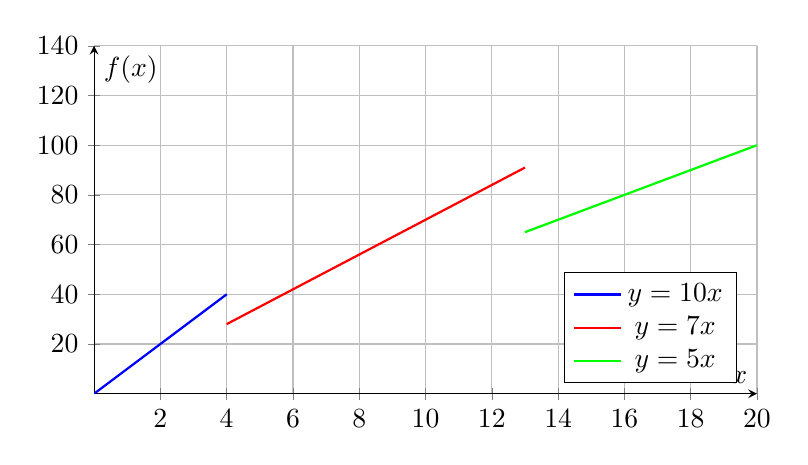
\begin{tikzpicture}
        \begin{axis}[
            axis lines = middle,
            xlabel = $x$, ylabel = {$f(x)$},
            xmin = 0, xmax = 20,
            ymin = 0, ymax = 140,
            xtick distance={2}, ytick distance={20},
            width = 10cm, height = 6cm,
            grid = both,
            legend pos = south east, % Positions the legend
        ]
            \addplot[blue, thick, domain=0:4, samples=100] {10 *x};
            \addlegendentry{$y = 10x$}

            \addplot[red, thick, domain=4:13, samples=100] {7 * x};
            \addlegendentry{$y = 7x$}

            \addplot[green, thick, domain=13:20, samples=100] {5 * x};
            \addlegendentry{$y = 5x$}
        \end{axis}
    \end{tikzpicture}
\end{figure}
\\
Just throwing these into a piecewise function would create a valid function, but one that doesn't represent the situation given. For it to represent the provided situation, the lines need to be connected. Let's examine why.

If $4$ hours passed, and $10$ dollars were given out every hour, then $40$ dollars were given out.

When the fifth hour passes, the piecewise function moves to the next equation, which we've currently assigned as $7x$. Plugging $x = 5$ to $7x$ gives $7 \times 5 = 35$. That's $5$ dollars less than what was given out in the first $4$ hours.

Since the amount given out in the fifth hour must add to the amount already given on the first $4$, we expect the amount after $5$ hours (i.e. $f(5)$) to be $47$ dollars.
\clearpage
You may think, "just shift the function up $12$ units ($y = 7x + 12$). Doing that gets us up to the $47$ we expect ($35 + 12 = 47$)." Although this \textit{would} work, it requires that you know how much was given out at the fourth hour.

Of course you can do that in this example. It's easy. But something like the one below would not be very easy to determine:
\begin{itemize}
    \item $\sin\left(\pi x\right)+\tan\left(\frac{x}{2}\right)$ acts on $x \in \left[-\frac{\pi}{13}, \frac{\pi}{9} \right]$
    \item $\tan\left(\frac{\pi^{2}x}{22}\right)$ acts on $x \in \left(\frac{\pi}{9}, \frac{\pi}{2}\right]$
\end{itemize}
The solution to that looks like this if you're curious:
\[
g(x) = 
\begin{cases}
    \sin\left(\pi x\right)+\tan\left(\frac{x}{2}\right) & 
    x \in \left[-\frac{\pi}{13}, \frac{\pi}{9} \right] \\
    %
    \tan\left(\frac{\pi^{2}\left(x-\frac{\pi}{9}\right)}{22}\right)+\sin\left(\frac{\pi^{2}}{9}\right)+\tan\left(\frac{\pi}{18}\right) & 
    x \in \left(\frac{\pi}{9}, \frac{\pi}{2}\right]
\end{cases}
\]
\vspace{-0.5cm}
\begin{figure}[ht]
    \centering
    \caption{Super Hard Problem (Scale: $\frac{\pi}{8}$)}
    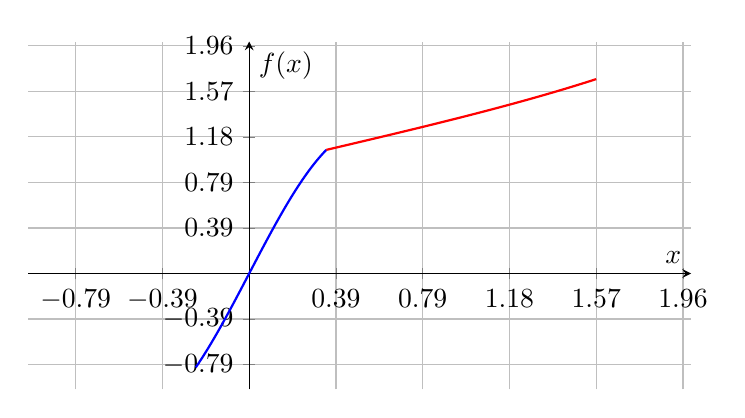
\begin{tikzpicture}
        \begin{axis}[
            axis lines = middle,
            xlabel = $x$, ylabel = {$f(x)$},
            xmin = -1, xmax = 2,
            ymin = -1, ymax = 2,
            xtick distance={pi / 8}, ytick distance={pi / 8},
            width = 10cm, height = 6cm,
            grid = both,
            legend pos = north east, % Positions the legend
            trig format plots=rad
        ]
            \addplot[blue, thick, domain=-(pi / 13):(pi / 9), samples=100] {sin(pi * x) + tan(x / 2)};
            \addplot[red, thick, domain=(pi / 9):(pi / 2), samples=100] {tan((pi^2 * (x - (pi / 9))) / 22) + sin(pi^2 / 9) + tan(pi / 18)};
        \end{axis}
    \end{tikzpicture}
\end{figure}
\clearpage
\subsection{The Correct Way To Do It}
Let's go back to the problem we were working on.

Instead of predicting or calculating how much we should add or subtract, we can literally move the entire function using vertical and horizontal transformations. 

In this case, we know that $y = 10x$ up until $x = 4$.

We're already given that $x = 4$, and $10 \times 4 = 40$, meaning $y = 40$.

What's left is to apply those transformations ($4$ right and $40$ up) to $7x$.

That gives: $y = 7(x - 4) + 40$.

This method does not rely on any calculations. All you need is the right-most edge of the bound ($4$ in this case) and the value of the equation at that bound ($40$ in this case). The same can be done for the last function.

In the first $4$ hours, the bank gave out $40$ dollars. In the next $9$ hours, the bank gave out $7 \times 9 = 63$ dollars. That means the total amount given is $40 + 63 = 103$ dollars.

We also know that the right-most boundary of the second equation is $x = 13$. That means we need to transform $5x$ 13 units to the right and $103$ units up, giving $y = 5(x - 13) + 103$.

Putting that all together gives the piecewise function and graph below:
\begin{center}
    \raisebox{0.5cm}{%
        \begin{minipage}[c]{0.48\textwidth}
            \centering
            \[
            g(x) = 
            \begin{cases}
                10x & x \in [0, 4] \\
                7(x - 4) + 40 & x \in (4, 13] \\
                5(x - 13) + 103 & x \in (13, \infty)
            \end{cases}
            \]
        \end{minipage}%
    }
    \begin{minipage}[c]{0.48\textwidth}
        \centering
        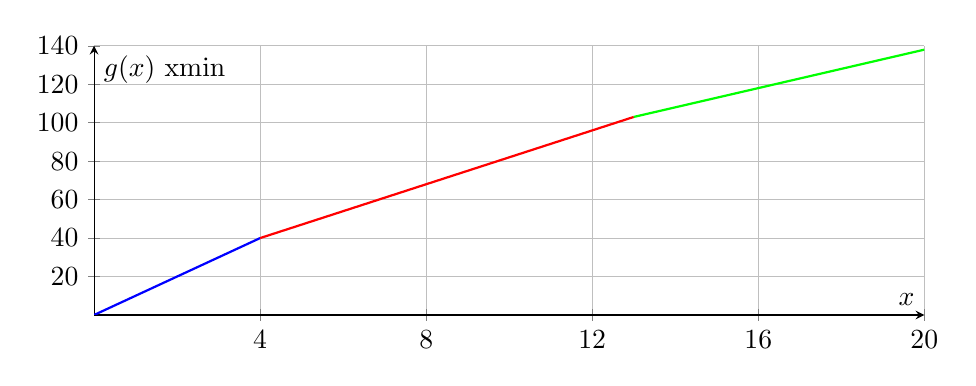
\begin{tikzpicture}
            \begin{axis}[
                axis lines = middle,
                xlabel = $x$, ylabel = {$g(x)$}
                xmin = 0, xmax = 20,
                ymin = 0, ymax = 140,
                xtick distance={4}, ytick distance={20},
                width = \linewidth,   % scale to the minipage width
                height = 5cm,
                grid = both,
                legend pos = south east,
            ]
                \addplot[blue, thick, domain=0:4, samples=100] {10 * x};
                \addplot[red, thick, domain=4:13, samples=100] {7 * (x - 4) + 40};
                \addplot[green, thick, domain=13:20, samples=100] {5 * (x - 13) + 103};
            \end{axis}
        \end{tikzpicture}
    \end{minipage}
\end{center}
\clearpage
\section{Jump Discontinuity}
Up to this point, we've been working with functions that continue cleanly from one another. To illustrate this point, I'll use another example. For those of you also taking physics, this sort of example may look familiar:
\begin{problem}
    Janet is a frequent runner and takes the same route to her friend's house every day. On her daily runs, she:
    \begin{itemize}
        \item Runs $1000\,m$ in $30$ minutes.
        \item Rests for $5$ minutes.
        \item Runs $750\,m$ in $30$ minutes.
        \item Rests for $10$ minutes.
        \item Runs $1200\,m$ in $45$ minutes.
    \end{itemize}
    Create a piecewise function and a Velocity vs. Time graph (VT Graph) representing Janet's velocity.
\end{problem}
For those who haven't taken physics, a Velocity vs. Time graph is just like a normal function but the $x$-axis is time $t$ and the $y$-axis is velocity $v$.

Also, instead of using $f(x)$ or $g(x)$, I'll be using $v(t)$, a velocity function with time (in minutes) as the independent variable.

We're not given any velocities, but we can find them quickly. Velocity is calculated by dividing the distance traveled by the time it took to travel that distance. For example, if you drove $30$ miles in $2$ hours then you were going $30\,mi / 2\,hr = 15\,mi/hr$. 

Using the equation $v = \frac{\Delta s}{\Delta t}$ ($s$ stands for change in position btw), we get:
\begin{align*}
    v_1 &= \frac{1000}{30} &
    v_2 &= \frac{0}{5} &
    v_3 &= \frac{750}{30} &
    v_4 &= \frac{0}{10} & 
    v_5 &= \frac{1200}{45} \\
    %
    v_1 &= \frac{100}{3} &
    v_2 &= 0 &
    v_3 &= 25 &
    v_4 &= 0 &
    v_5 &= \frac{80}{3}
\end{align*}
\clearpage
We don't have any variables here, so there's nothing to line up. That means we can create the piecewise function and graph right now:
\begin{center}
    \begin{minipage}[c]{0.48\linewidth}
        \[
            v(t) = 
            \begin{cases}
            \frac{100}{3} & t \in [0, 30] \\
            0 & t \in (30, 35] \\
            25 & t \in (35, 65] \\
            0 & t \in (65, 75] \\
            \frac{80}{3} & t \in (75, 120]
            \end{cases}
        \]
    \end{minipage}
    \begin{minipage}[c]{0.48\textwidth}
        \centering
        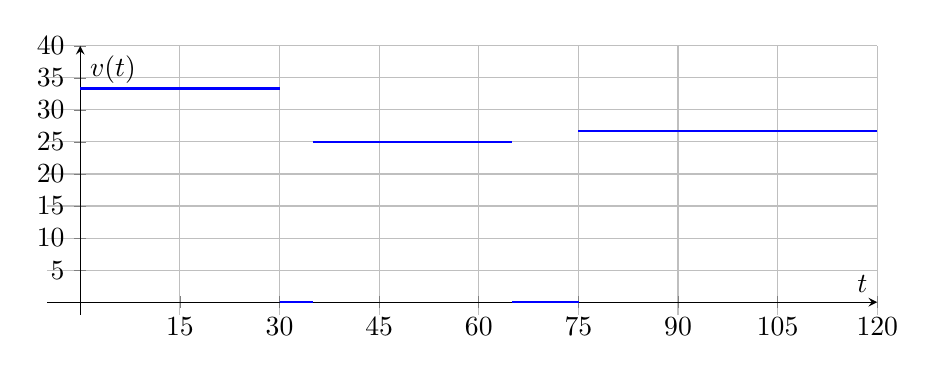
\begin{tikzpicture}
            \begin{axis}[
                axis lines = middle,
                xlabel = $t$, ylabel = {$v(t)$},
                xmin = -5, xmax = 120,
                ymin = -2, ymax = 40,
                xtick distance={15}, ytick distance={5},
                width = \linewidth,   % scale to the minipage width
                height = 5cm,
                grid = both,
                legend pos = south east,
            ]
                \addplot[blue, thick, domain=0:30, samples=100] {100 / 3};
                \addplot[blue, thick, domain=30:35, samples=100] {0};
                \addplot[blue, thick, domain=35:65, samples=100] {25};
                \addplot[blue, thick, domain=65:75, samples=100] {0};
                \addplot[blue, thick, domain=75:120, samples=100] {80 / 3};
            \end{axis}
        \end{tikzpicture}
    \end{minipage}
\end{center}
This function doesn't smoothly transition like with the bank example. It breaks off and continues in different places. It jumps from $v = 35$ all the way down to $v = 0$, hence why it's called a "jump" discontinuity. This is \textbf{not} continuous. Also... $25$ minutes per minute? Dayum she's slow. But that's beside the point.
\clearpage
\section{Removable Discontinuity}
A removable discontinuity is a less obvious than a jump discontinuity. The function may \textit{look} continuous, but it'll have a hole somewhere. I won't spend too much time on this because it's solved almost identically to regular piecewise functions. In fact, I can actually use a previous example to demonstrate this.

Here was the result from that bank example:
\begin{center}
    \raisebox{0.5cm}{%
        \begin{minipage}[c]{0.48\textwidth}
            \centering
            \[
            g(x) = 
            \begin{cases}
                10x & x \in [0, 4] \\
                7(x - 4) + 40 & x \in (4, 13] \\
                5(x - 13) + 103 & x \in (13, \infty)
            \end{cases}
            \]
        \end{minipage}%
    }
    \begin{minipage}[c]{0.48\textwidth}
        \centering
        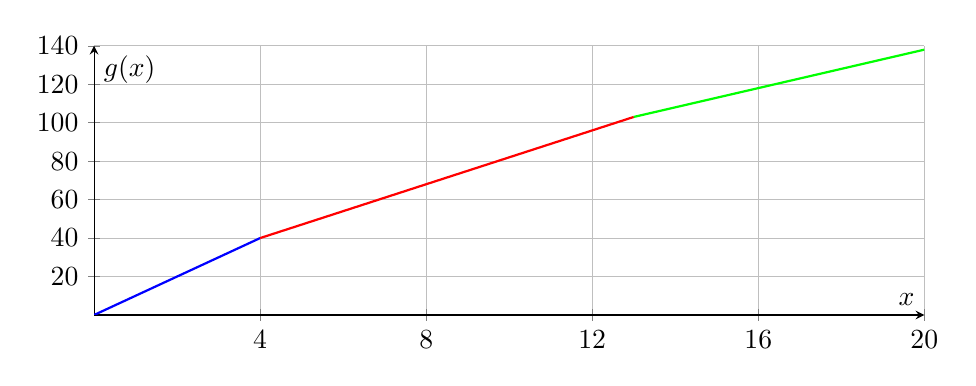
\begin{tikzpicture}
            \begin{axis}[
                axis lines = middle,
                xlabel = $x$, ylabel = {$g(x)$},
                xmin = 0, xmax = 20,
                ymin = 0, ymax = 140,
                xtick distance={4}, ytick distance={20},
                width = \linewidth,   % scale to the minipage width
                height = 5cm,
                grid = both,
                legend pos = south east,
            ]
                \addplot[blue, thick, domain=0:4, samples=100] {10 * x};
                \addplot[red, thick, domain=4:13, samples=100] {7 * (x - 4) + 40};
                \addplot[green, thick, domain=13:20, samples=100] {5 * (x - 13) + 103};
            \end{axis}
        \end{tikzpicture}
    \end{minipage}
\end{center}
This function is continuous because there are no gaps. But what if we changed the inequality $x \in [0, 4]$ to $x \in [0, 4)$?

If we did that, the function would begin at $0$, continue all the way up to $3.99999\dots$, then skip $4$ to go to $4.00000\dots 1$ and continue as normal. Making some substitutions would help visualize what's going on.
\begin{align*}
    f(3.9) &= 39 \\
    f(4) &= undefined \\
    f(4.1) &= 40.7
\end{align*}
\clearpage
Since the function has nothing defined for $x = 4$ (i.e. it's skipped), it's labeled as undefined. The function $f$ has no value at $x = 4$. On a graph, that is usually labeled by an open circle.

With that change, the piecewise function and graph now looks like this:
\begin{center}
    \raisebox{0.5cm}{%
        \begin{minipage}[c]{0.48\textwidth}
            \centering
            \[
            g(x) = 
            \begin{cases}
                10x & x \in [0, 4) \\
                7(x - 4) + 40 & x \in (4, 13] \\
                5(x - 13) + 103 & x \in (13, \infty)
            \end{cases}
            \]
        \end{minipage}%
    }
    \begin{minipage}[c]{0.48\textwidth}
        \centering
        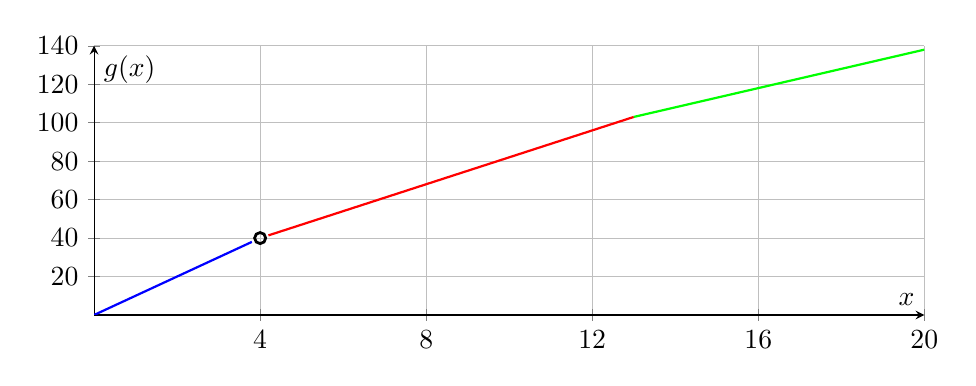
\begin{tikzpicture}
            \begin{axis}[
                axis lines = middle,
                xlabel = $x$, ylabel = {$g(x)$},
                xmin = 0, xmax = 20,
                ymin = 0, ymax = 140,
                xtick distance={4}, ytick distance={20},
                width = \linewidth,   % scale to the minipage width
                height = 5cm,
                grid = both,
                legend pos = south east,
            ]
                \addplot[blue, thick, domain=0:3.8, samples=100] {10 * x};
                \addplot[red, thick, domain=4.2:13, samples=100] {7 * (x - 4) + 40};
                \addplot[green, thick, domain=13:20, samples=100] {5 * (x - 13) + 103};
                \addplot[only marks, mark=o, mark options={draw=black, fill=white, line width=1pt}, mark size=2pt] coordinates {(4, 40)};
            \end{axis}
        \end{tikzpicture}
    \end{minipage}
\end{center}